\section{Memorandum to the Chief Operations Officer of HiMCM}

\noindent\textbf{To:} Chief Operations Officer, HiMCM\\
\textbf{From:} Team 19678\\
\textbf{Date:} November 16, 2026\\
\textbf{Subject:} Cooling strategy for the Grove Hall bus shelter

We recommend the Fan as Grove Hall's primary cooling system. Consider the Large Evaporative Cooler for peak heat if resources allow. In the humid summer conditions we modeled, the Fan brought passengers within our comfort range using no water and just 0.25 kWh of electricity in one hour. In Boston's hot-dry case, the shelter was already comfortable with the equipment off. The Large Evaporative Cooler provided additional relief during the peak-heat case.

Grove Hall was one of six bus and rail waiting areas in our broader study of 12 sites across Boston, Dallas, and Phoenix. Using summer 2025 weather data, we compared a fan, two sizes of evaporative cooler, and no cooling. At an open-sided shelter, passenger comfort depends on air temperature, humidity, and airflow. A fan moves air across the skin. An evaporative cooler lowers the air temperature and adds humidity as the supply air mixes with outdoor air. To compare what passengers would experience, we used Standard Effective Temperature (SET), which expresses the combined effects of temperature, humidity, airflow, and radiant heat on a common temperature scale. The figures below are estimates on that scale. We used 23--26$^{\circ}$C as our comfort range.

In the hot-humid case, the Fan brought estimated conditions from 27.66$^{\circ}$C to 25.09$^{\circ}$C. All three devices reached the target. The Fan used 90\% less electricity than the Large Evaporative Cooler and saved about 44 liters of water in the modeled hour. It also had the lowest reference purchase price at \$1,499, compared with \$4,159 for the Small Evaporative Cooler and \$4,939 for the Large Evaporative Cooler~\cite{aireye_20_price,portacool_2000,portacool_4000}. In the hot-dry case, the shelter started at 24.44$^{\circ}$C, and all three devices pushed conditions below the lower end of the comfort range.

Peak heat presented a harder decision. With the equipment off, estimated conditions reached 30.77$^{\circ}$C. The Fan brought that down to 29.07$^{\circ}$C and the Large Evaporative Cooler to 28.57$^{\circ}$C. The Large Evaporative Cooler led the comfort benchmark. When we tested limits on purchase cost, electricity, and water at Grove Hall, the Fan was the best feasible option across the three scenarios. The practical trade-off is what it took to gain that last half-degree during the peak hour: 2.50 kWh of electricity, ten times the Fan's consumption, and roughly 81 liters of evaporated water. Even then, conditions remained above the comfort target.

\medskip
\noindent\textbf{Key Recommendations}
\begin{enumerate}
\setlength{\itemsep}{2pt}
\setlength{\parsep}{0pt}
\item \textbf{Leave cooling off when the shelter is already comfortable.} In Boston's hot-dry scenario, the uncooled waiting area was within the target range, and all three systems would have cooled it below that range. Under those conditions, operators can save electricity and water simply by leaving the equipment off.
\item \textbf{Use the Fan as Grove Hall's primary source of relief.} In humid heat, the Fan brought passengers within the comfort range using 90\% less electricity than the Large Evaporative Cooler and no water. As long as the Fan meets that target, there is little reason to run either evaporative cooler.
\item \textbf{Consider the Large Evaporative Cooler for peak heat if resources allow.} The Large Evaporative Cooler provided about half a degree of extra relief at peak heat. Across the modeled hours, it requires \$4,939 upfront, 2.50 kWh per hour, and a water allowance of about 84.1 liters for the highest-use hour.
\item \textbf{Provide access to air-conditioned shelter during hazardous heat.} Even with the Large Evaporative Cooler running, Grove Hall remained above the comfort target during peak heat. Identify a nearby air-conditioned place where passengers can wait and post clear directions at the stop.
\end{enumerate}

\clearpage
\phantomsection
\addcontentsline{toc}{section}{Public Blog Post}
\begin{figure}[H]
    \centering
    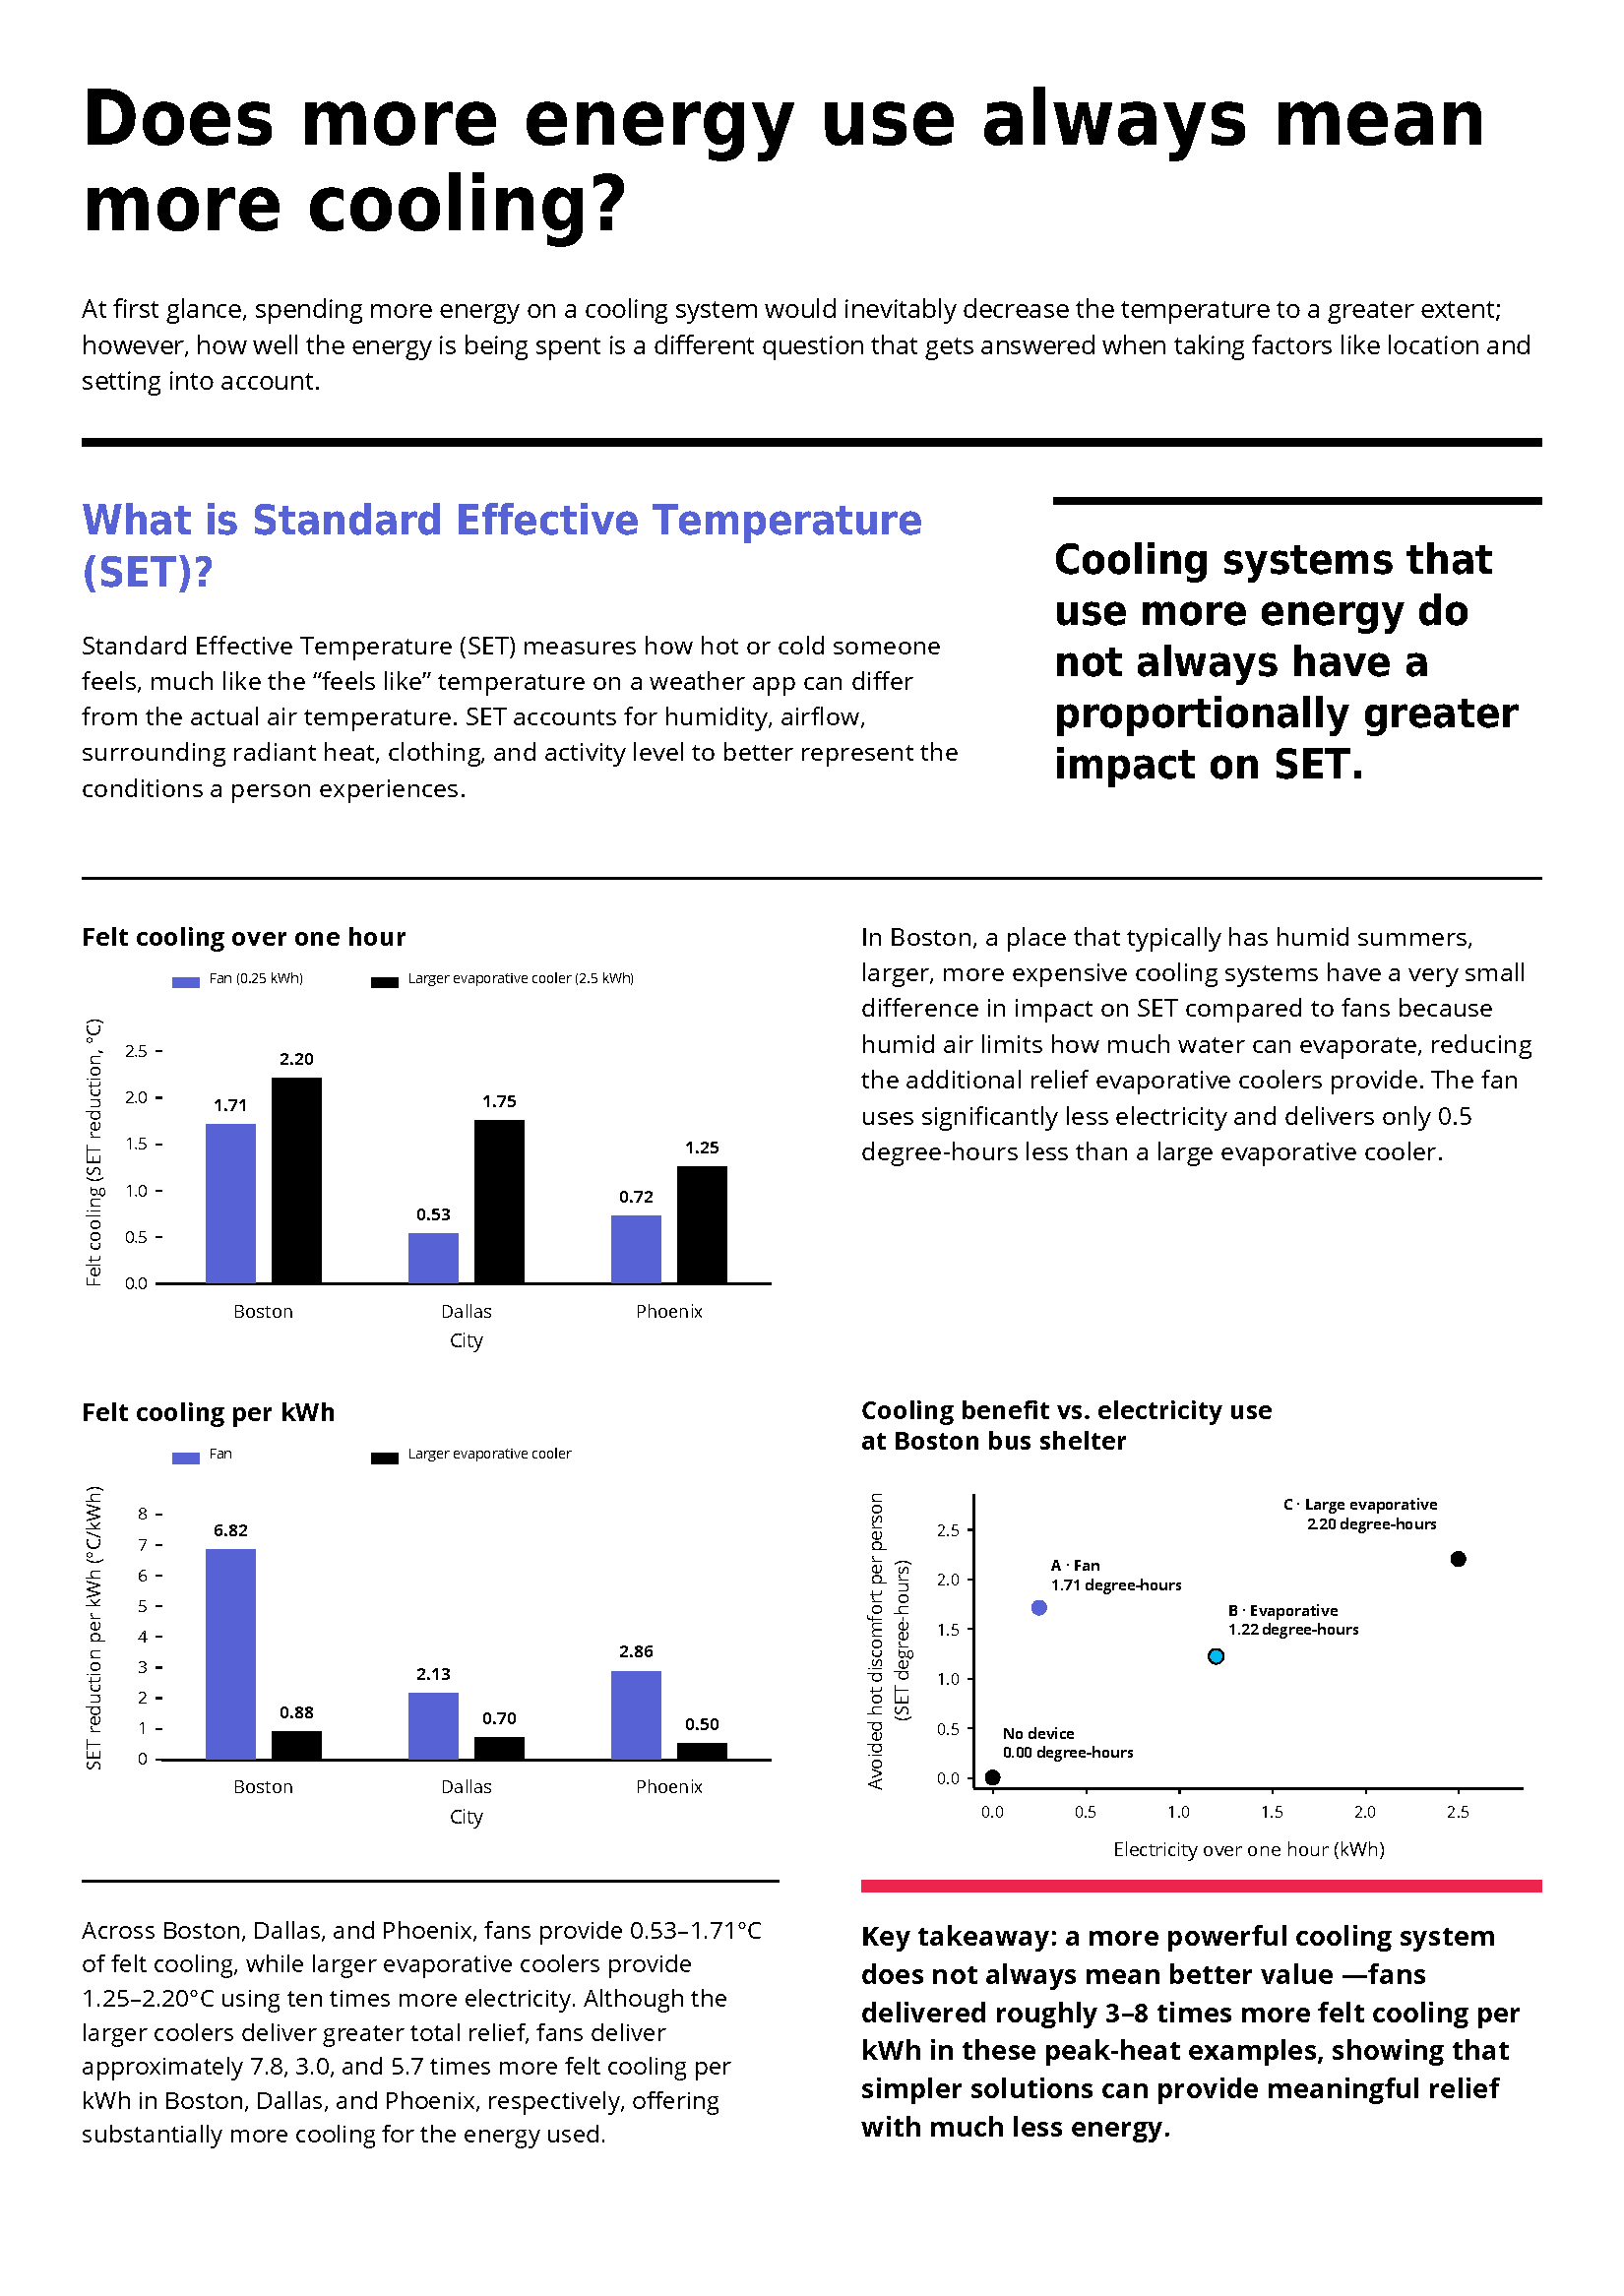
\includegraphics[width=0.88\linewidth]{Images/HiMCM26_BlogPost_Designed.pdf}
    \label{fig:blog-post}
\end{figure}